\documentclass{exam}
\usepackage[utf8]{inputenc}
\usepackage{lmodern}
\usepackage{microtype}

% \usepackage[parfill]{parskip}
\usepackage[dvipsnames]{xcolor}
\usepackage{amsmath}
\usepackage{amsfonts}
\usepackage{amsthm}
\usepackage{siunitx}
\DeclareSIUnit\year{yr}
\DeclareSIUnit\foot{ft}
\DeclareSIUnit\litre{\liter}

\usepackage{skull}

\usepackage{pgfplots}
\usepgfplotslibrary{polar}
\pgfplotsset{compat=1.11}
\usepgfplotslibrary{statistics}
\usepackage{graphicx}
\usepackage{sidecap}
\sidecaptionvpos{figure}{c}
\usepackage{float}
\usepackage{gensymb}
\usepackage{tkz-euclide}
\usetkzobj{all}
\usepackage{commath}
\usepackage{hyperref}
\usepackage{enumitem}
\usepackage{wasysym}
\usepackage{multicol}
\usepackage{mathtools}
\usepackage{tcolorbox}
\usepackage{tabularx}
\usepackage[version=4]{mhchem}
\usepackage{changepage}
\usepackage{listings}
\lstset{basicstyle=\ttfamily\linespread{0.8}\small}

\renewcommand*{\thefootnote}{\fnsymbol{footnote}}

\newtheorem*{thm}{Theorem}
\newtheorem*{iden}{Identity}
\newtheorem*{lemma}{Lemma}
\newtheorem{obs}{Observation}
\theoremstyle{definition}
\newtheorem*{defn}{Definition}
\newtheorem*{ex}{Example}
\newtheorem{con}{Construction}
\newtheorem*{alg}{Algorithm}

\newtheoremstyle{break}
  {\topsep}{\topsep}%
  {\itshape}{}%
  {\bfseries}{}%
  {\newline}{}%
\theoremstyle{break}
\newtheorem*{bthm}{Theorem}

% russian integral
\usepackage{scalerel}
\DeclareMathOperator*{\rint}{\scalerel*{\rotatebox{17}{$\!\int\!$}}{\int}}

% \DeclareMathOperator*{\rint}{\int}

\pgfplotsset{vasymptote/.style={
    before end axis/.append code={
        \draw[densely dashed] ({rel axis cs:0,0} -| {axis cs:#1,0})
        -- ({rel axis cs:0,1} -| {axis cs:#1,0});
    }
}}

% \pointsinrightmargin
\boxedpoints
\pointname{}

\newcommand{\questioA}{\question[\texttt{\textbf{\color{Cerulean} A}}]}
\newcommand{\questioM}{\question[\texttt{\textbf{\color{PineGreen} M}}]}
\newcommand{\questioE}{\question[\texttt{\textbf{\color{WildStrawberry} E}}]}
\newcommand{\questioS}{\question[\texttt{\textbf{\color{Goldenrod} S}}]}
\newcommand{\questioO}{\question[\texttt{\textbf{\color{BurntOrange} O}}]}

\newcommand{\parA}{\part[\texttt{\textbf{\color{Cerulean} A}}]}
\newcommand{\parM}{\part[\texttt{\textbf{\color{PineGreen} M}}]}
\newcommand{\parE}{\part[\texttt{\textbf{\color{WildStrawberry} E}}]}
\newcommand{\parS}{\part[\texttt{\textbf{\color{Goldenrod} S}}]}
\newcommand{\parO}{\part[\texttt{\textbf{\color{BurntOrange} O}}]}

\newcommand{\subparA}{\subpart[\texttt{\textbf{\color{Cerulean} A}}]}
\newcommand{\subparM}{\subpart[\texttt{\textbf{\color{PineGreen} M}}]}
\newcommand{\subparE}{\subpart[\texttt{\textbf{\color{WildStrawberry} E}}]}
\newcommand{\subparS}{\subpart[\texttt{\textbf{\color{Goldenrod} S}}]}
\newcommand{\subparO}{\subpart[\texttt{\textbf{\color{BurntOrange} O}}]}

\newcommand{\mainHeader}[2]{\section*{NCEA Level 2 Mathematics\\#1. #2}}
\newcommand{\mainHeaderHw}[2]{\section*{NCEA Level 2 Mathematics (Homework)\\#1. #2}}
\newcommand{\seealso}[1]{\begin{center}\emph{See also #1.}\end{center}}
\newcommand{\drills}[1]{\begin{center}\emph{Drill problems: #1.}\end{center}}
\newcommand{\basedon}[1]{\begin{center}\emph{Notes largely based on #1.}\end{center}}


\begin{document}

\mainHeaderHw{15}{Kinematics and Rates of Change}
\subsection*{Reading}
\begin{center}
\begin{tcolorbox}[width=0.8\textwidth,colback={white},title={\textbf{Go and watch...}},colbacktitle=black,coltitle=white]
  \textcolor{black}{\url{https://www.youtube.com/watch?v=pI62ANEGK6Q}}
\end{tcolorbox}
\end{center}

\noindent
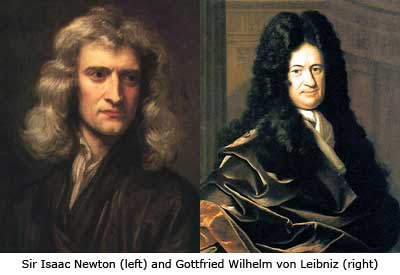
\includegraphics[width=0.5\textwidth]{newton-leibniz}
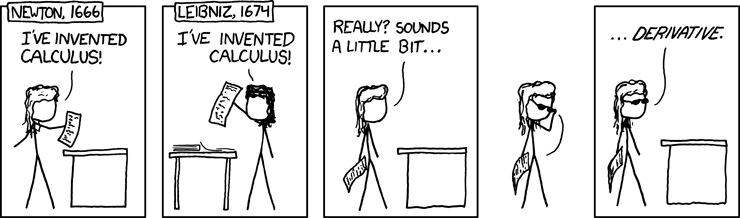
\includegraphics[width=0.5\textwidth]{newton-leibniz-2}

Maybe it's time to tell the story of Isaac Newton and Gottfried Wilhelm Leibniz. If you've ever studied calculus, you know it was created independently by Newton and Leibniz. Few of us appreciate the full fury of the priority dispute behind that.

Newton was born in 1642, Leibniz four years later. Calculus is a means for calculating the way quantities vary with each other, rather than just the quantities themselves. The bare bones of that idea had been hatching (since the Greeks) before either Newton or Leibniz was born. But they each wrote a full system of calculus.

In 1665 Newton created his somewhat clumsy method of fluxions. He feared criticism and sat on his work 'til 1704. Then he published it as an appendix to his book on Optiks (the behaviour of light). The odd thing is, he began his fight with Leibniz long before he published anything. Leibniz wrote his calculus around 1673, and he used the notation we still use today -- derivatives expressed as dy/dx, and so on. He too sat on his work for a long time. He published it in 1684 (still twenty years ahead of Newton!).

A surprised Newton took the offensive. But both men had cronies egging them on. Johann Bernoulli, who used Leibniz's calculus to maximize functions, goaded Leibniz into fighting Newton. Newton was surrounded by toadies whom Leibniz called the enfants perdus, the lost children. Newton choreographed the attack, and they carried the battle. They accused Leibniz of plagiarism, a charge that falls apart when you trace the details. In the end, Newton's campaign was effective and damaging. He emerged with the credit. But when people like Leonard Euler and the Bernoullis erected the field of applied analysis, they used Leibniz's calculus.

Leibniz worked in an astonishing variety of fields. He was first to state the conservation of energy. He worked for a reunification of Catholics and Protestants. That may well've been fed by his optimistic metaphysics. It was he who claimed we live in the best of all possible worlds. Voltaire, born when both Newton and Leibniz were on in years, wouldn't stand still for that. While his mistress, Emily de Breteuil, translated Newton's Principia into French, Voltaire wrote Candide. And Candide's friend Dr. Pangloss made vicious sport of Leibniz's optimism.

Leibniz died poor and dishonored, while Newton was given a state funeral. Yet history validates Leibniz. For as time passes, so does the potency of Newton's assault. And Leibniz gradually finds his place as one of the great thinkers of all time.

\begin{flushright}
  Adapted from \url{http://www.uh.edu/engines/epi1375.htm}.
\end{flushright}

\clearpage
\subsection*{Questions}
All distances are given in \si{\metre}, and all times in \si{\second}, unless otherwise stated.
\begin{questions}
  \question A particle moves in space along a single axis, with velocity function $ v(t) = t^2 + t - 12 $ (where $ t $ is measured from some
            arbitrary starting point).
    \begin{parts}
      \part What is the acceleration of the particle at $ t = \SI{10}{\second} $?
      \part The particle is closest to the origin at $ t = \SI{3}{\second} $.
        \begin{subparts}
          \subpart By considering $ v(t) $, show that $ t = 3 $ is indeed a turning point for the graph of the position function $ x(t) $ of the particle.
          \subpart If the minimum distance between the particle and the origin is \SI{300}{\metre}, calculate the distance from the particle
                   to the origin at $ t = \SI{10}{\second} $.
        \end{subparts}
    \end{parts}
  \question A cubic equation is a polynomial of degree three --- that is, a function
            of the form $ f(x) = ax^3 + bx^2 + cx + d $ where $ a \neq 0 $. Recall that
            a critical point is a point $ x $ where $ f'(x) = 0 $, or $ f'(x) $ is undefined.
            \begin{subparts}
              \subpart Sketch examples of a cubic function with zero, one, and two critical points.
              \subpart Prove that a cubic function can have a maximum of two critical points.
            \end{subparts}

\end{questions}

\end{document}
